\chapter{実装}
本章では,ADLoggerシステムの実装について述べる.
はじめに実装環境について述べ,ついでタスク別時間記録モジュール,必要時間予測モジュールについて説明する.

\section{実装環境}
本節では,本システムにおける実装環境について説明する.本システムはiPhoneアプリケーションであり,実装言語にはSwiftを使用している.
サーバサイド兼データベースには,MBaaS (Mobile Backend as a Service)であるBack4App~\cite{back4app}を利用している.

\section{クライアント側実装}
クライアントはiPhoneアプリケーションであり,Swiftによって実装した.
タスク別時間記録モジュール,必要時間予測モジュールについて説明する.

\subsection{タスク別時間記録モジュール}
本節ではタスク別時間記録モジュールについて説明する.
タスク別時間記録モジュールはユーザが行動したタスク及び時間を記録するモジュールである.
メイン画面のUIButton``TIMER"を押すと,ストップウォッチ画面に遷移する.(図~\ref{fig:stopwatch}参照)
UIButton``START"を押すとUIButtonが``STOP"に書き換えられた後,
上段に配置したUILabel``00:00:00"から “hh:mm:ss”の書式で書き換えられ経過時間が表示される.

\begin{figure}[ht]
\begin{center}
\begin{tabular}{c}

	\begin{minipage}[b]{0.5\linewidth}
	\begin{center}
		\fbox{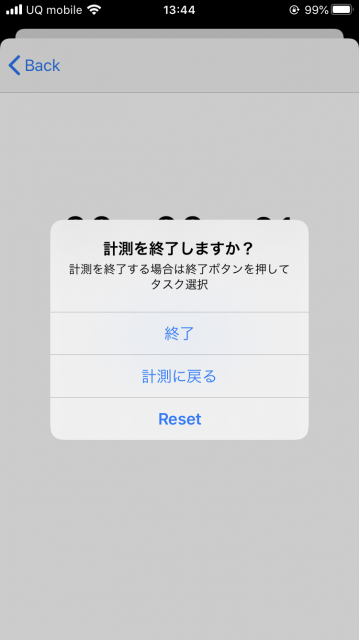
\includegraphics[width=5cm]{images/6/salert.png}}
		\caption{計測に関する選択}
		\label{fig:salert}
	\end{center}
  	\end{minipage}
	
	\begin{minipage}[b]{0.5\linewidth}
	\begin{center}
		\fbox{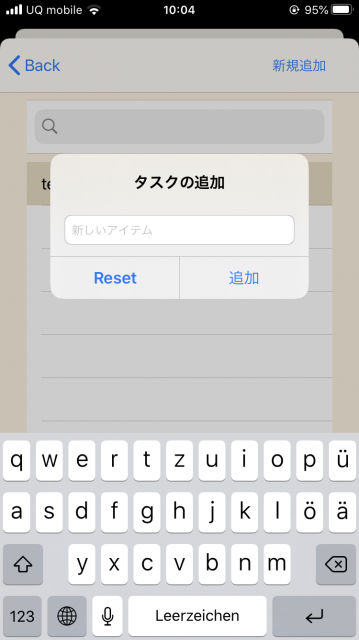
\includegraphics[width=5cm]{images/6/newtask.png}}
		\caption{新規追加}
		\label{fig:newtask}
	\end{center}
  	\end{minipage}
	
	\\
	
	\begin{minipage}[b]{0.5\linewidth}
	\begin{center}
		\fbox{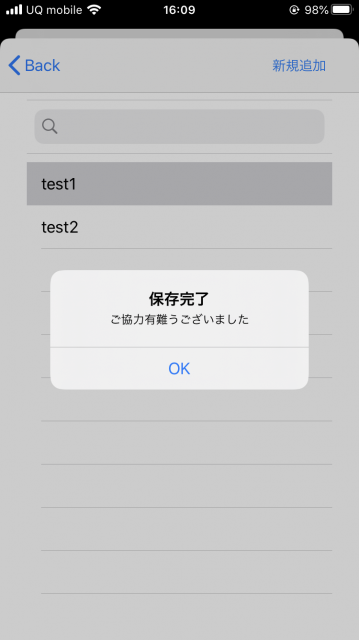
\includegraphics[width=5cm]{images/6/saved.png}}
		\caption{保存完了}
		\label{fig:saved}
	\end{center}
  	\end{minipage}

\end{tabular}
\end{center}
\end{figure}

再度UIButtonを押すとタスク別時間記録モジュールによって図~\ref{fig:salert}のようなUIAlertControllerが表示される.
このUIAlertControllerは,``終了"と``計測に戻る"と``Reset"の3つの選択肢を持っている.

``計測に戻る"を選択すると,UIButtonが``STOP"から``START"に書き換えられた後,上記の経過時間測定と同じ方法でカウントアップが再開される.
``Reset"を選択すると,上段の数字はカウントアップを終了しUILabelが``00:00:00"に書き換えられる事でリセット状態となる.
``終了"を選択すると現在のUILabelの値をInt型で変換した後,型で渡し,タスク選択画面へ遷移する.

タスク選択画面ではUITableViewで過去記録した事のあるタスク名が表示される.
各UITableViewCellに表示されているタスク名は,端末内のUserDefaultsにString型の配列として保存されている.
``新規追加"ボタンを押すと,UIAlertControllerが表示される(図~\ref{fig:newtask}).
このUIAlertControllerにはtextFieldが内蔵されており,新規タスクを記入しOKを押すとString型の配列に入力したtextFieldの値が新規タスクとして追加される.
UITableViewCellをタップすると記録した値がサーバーに送信され,保存が成功した事を示すUIAlertControllerが表示される(図~\ref{fig:saved}).
サーバに送られる値は表~\ref{tb:study_record}の通りである.

\begin{table}[htb]
\begin{center}
  \begin{tabular}{|l|l|} \hline
    サーバに送る値 & 型 \\ \hline
    ユーザID & PFUser型(サーバ指定のユーザ型) \\
    タスク名 & String型 \\
    記録時間(秒) & Int型 \\
    記録日時 & Date型 \\
	\hline
  \end{tabular}
  \caption{サーバに送信する値}
  \label{tb:study_record}
\end{center}
\end{table}

\subsection{必要時間予測モジュール}
続いて,必要時間予測モジュールについて説明する.
%ーーーーーーーーここから!ーーーーーーーーーーーーーーーーーーーー

\section{まとめ}
本章では,ADLoggerシステムの実装について述べた.
次章では,本システムで得られたデータから動機づけの向上を評価し,考察について述べる.
